\section{Experiments}

We evaluate the performance of the proposed slice sampler in the setting of
covariate dependent density estimation.  We assume 
the statistical
model in Eq.~\ref{eqn:mixmod} and consider a univariate Gaussian
distribution as the data generating distribution.  We use both synthetic and
real data sets in our experiments and compare the slice sampler to a Gibbs
sampler for a finite approximation to the model (see the supplement
for details of the model and sampler) and to the original SNGP sampler.
We assess the mixing
characteristics of the sampler using the integrated autocorrelation time $\tau$ of the
number of clusters used by the sampler at each iteration after a burn-in
period, and by the predictive quality of the collective samples on held-out
data.  The integrated autocorrelation time
of samples drawn from an MCMC algorithm
controls the Monte Carlo error inherent in a sample drawn from the MCMC
algorithm.  It can be shown that in a set of $T$ samples from the MCMC
algorithm, there are in effect only $T/(2\tau)$ ``independent'' samples.
Therefore, lower values of $\tau$ are deemed better. We obtain an estimate 
$\hat{\tau}$ of the integrated autocorrelation time following 
\cite{KalliGriffinWalker:2011}.

%The integrated autocorrelation time, denoted $\tau$, has become a common 
%measure of the mixing quality of MCMC samplers \cite{KalliGriffinWalker:2011}. % An estimate of
%$\tau$ is defined as
%\begin{equation}
%  \hat{\tau} = \frac{1}{2} + \sum_{l=1}^{C-1} \hat{\rho}_l
%  \label{eqn:iac}
%\end{equation}
%Here $\hat{\rho}_l$ is the estimated autocorrelation at lag $l$ and $C$ is a
%lag at which to truncate the sum.  As in \cite{KalliGriffinWalker:2011} we choose the maximum lag
%as $C = \min\{l : |\hat{\rho}_l < 2/\sqrt{M}\}$ which is the smallest lag that
%rejects the null hypothesis $H_0 : \rho_l = 0$ and $M$ is the number of samples
%drawn.  See \cite{KalliGriffinWalker:2011} for a complete
%discussion concerning this choice of $C$.  The integrated autocorrelation time
%of samples drawn from an MCMC algorithm
%controls the Monte Carlo error inherent in a sample drawn from the MCMC
%algorithm.  It can be shown that in a set of $M$ samples from the MCMC
%algorithm, there are in effect only $M/(2\tau)$ ``independent'' samples.
%Therefore, lower values of $\hat{\tau}$ are deemed better.
%In this paper we compute $\hat{\tau}$ for the number of used clusters, that is
%clusters with at least one observation allocated.

We assess the predictive performance of the collected samples from the various
algorithms by computing a Monte Carlo estimate of the predictive log-likelihood 
of a held-out data point under the model.  Specifically, for a held out point
$y^*$ we have
\begin{equation}
  \log p(y^*|y) \approx \frac{1}{T} \sum_{t=1}^T \log \left ( \sum_{m=1}^{M^{(t)}}
  w^{(t)}_m q \left ( y^*|\theta^{(t)}_m,\phi^{(t)}_m \right )  \right ).
  \label{eqn:logp}
\end{equation}
The weight $w^{(t)}_m$ is the probability of choosing atom $m$ for sample $t$.
We did not use the Rao-Blackwellized estimator to compute
Eq.~\ref{eqn:logp} for the slice sampler to achieve fair comparisons (see
the supplement for the results using the Rao-Blackwellized estimator).

% Updated 5-fold table
\begin{table}
  \centering
  \caption{Results of the samplers using different kernels.  Entries
  are of the form ``average predictive density / average number of clusters used /
  $\hat{\tau}$'' where two standard errors are shown in parentheses.  Results are 
  averaged over 5 hold-out data sets.}
  \vspace{3pt}
  \begin{tabular}{|c|c|c|c|}
    \hline
    & \textbf{Synthetic} & \textbf{CMB} & \textbf{Motorcycle} \\
    \hline
    Slice Box  & -2.70 (0.12) / 11.6 / 2442 & -0.15 (0.11) / 14.4 / 2465 & -0.90 (0.28) / 10.3 / 2414  \\
    \hline
    SNGP       & -2.67 (0.12) / 43.3 / 2488 & -0.22 (0.14) / 79.1 / 2495 & NA \\
    \hline
    Finite Box & -2.78 (0.15) / 11.7 / 2497 & -0.41 (0.14) / 18.2 / 2444 & -1.19 (0.16) / 16.4 / 2352  \\
    \hline
    Slice SE   & NA                         & -0.28 (0.07) / 14.7 / 2447 & -0.87 (0.28) / 8.2 / 2377 \\
    \hline
    Finite SE  & NA                         & -0.29 (0.05) / 9.5 / 2491 & -0.99 (0.19) / 7.3 / 2159 \\
    \hline
  \end{tabular}
  \label{tab:mcmc}
\end{table}


% Submitted table
%\begin{table}
%  \centering
%  \caption{Results of the samplers using different kernels.  Entries
%  are of the form ``average predictive density / average number of used clusters /
%  $\hat{\tau}$'' where one standard error is shown in parentheses.}
%  \vspace{3pt}
%  \begin{tabular}{|c|c|c|c|}
%    \hline
%    & \textbf{Synthetic} & \textbf{CMB} & \textbf{Motorcycle} \\
%    \hline
%    Slice Box  & -2.56 (0.13) / 11.4 / 2467 & -0.31 (0.10) / 13.3 / 2455 & -0.65 (0.49) / 10.3 / 2423  \\
%    \hline
%    SNGP       & -2.55 (0.15) / 26.7 / 2470 & -0.40 (0.20) / 66.6 / 2494 & NA \\
%    \hline
%    Finite Box & -2.69 (0.15) / 13.0 / 2498 & -0.42 (0.16) / 20.8 / 2432 & -1.03 (0.23) / 16.0 / 2333  \\
%    \hline
%    Slice SE   & NA & -0.36 (0.07) / 14.1 / 2446 & -0.52 (0.38) / 8.7 / 2386 \\
%    \hline
%    Finite SE  & NA & -0.34 (0.07) / 10.0 / 2498 & -0.78 (0.23) / 6.7 / 2142 \\
%    \hline
%  \end{tabular}
%  \label{tab:mcmc}
%\end{table}

% Original table
%\begin{table}
%  \centering
%  \caption{Results of the various algorithms using different kernels.  Entries
%  are of the form ``average predictive density / average number of used clusters /
%  $\hat{\tau}$'' where one standard error is shown in parentheses.}
%  \vspace{3pt}
%  \begin{tabular}{|c|c|c|c|}
%    \hline
%    & \textbf{Synthetic} & \textbf{CMB} & \textbf{Motorcycle} \\
%    \hline
%    Slice Box  & -2.56 (0.13) / 11.44 / 2467.39 & -0.31 (0.10) / 13.27 / 2454.81 & -0.65 (0.49) / 10.27 / 2423.47  \\
%    \hline
%    SNGP       & -2.55 (0.15) / 26.73 / 2470.43 & -0.40 (0.20) / 66.59 / 2493.85 & NA \\
%    \hline
%    Finite Box & -2.69 (0.15) / 13.00 / 2497.97 & -0.42 (0.16) / 20.76 / 2432.08 & -1.03 (0.23) / 15.97 / 2333.40  \\
%    \hline
%    Slice SE   & NA & -0.36 (0.07) / 14.06 / 2445.79 & -0.52 (0.38) / 8.66 / 2385.69 \\
%    \hline
%    Finite SE  & NA & -0.34 (0.07) / 10.00 / 2498.00 & -0.78 (0.23) / 6.65 / 2142.21 \\
%    \hline
%  \end{tabular}
%  \label{tab:mcmc}
%\end{table}


\subsection{Synthetic data}

We generated synthetic data from a dynamic mixture model with $12$
components (Figure \ref{fig:slicestats}).  Each component has an associated 
location, $\mu_k$, that can take
the value of any of ten uniformly spaced time stamps, $t_j \in [0,1]$.  The
components are active according to the kernel $K(x,\mu_k) = \idf{|x-\mu_k| <
.2}$ -- i.e. components are active for two time stamps around their location.
At each time stamp, $t_j$, we generate $60$ data points.  For each data point we choose 
a component, $k$, such that $\idf{|t_j-\mu_k| < .2}$ and then generate that
data point from a Gaussian distribution with mean $\mu_k$
and variance $10$.  We use $50$ of the generated data points
per time stamp as a training set and hold out $10$ data points for prediction.

Since the SNGP is a special case of the normalized KGaP, we compare the finite 
and slice
samplers, which are both conditional samplers, to the original marginal sampler
proposed in \cite{Rao:Teh:2009}.  We use the basic version of the SNGP that 
uses fixed-width kernels, as we assume fixed width kernel functions for simplicity.
The implementation of the SNGP sampler we used also only allows for fixed
component variances, so we fix all $\phi_k = 1/10$, the true data generating
precision.  We use the true kernel function that was used to generate the data 
as the kernel for the normalized KGaP model.

We ran the slice sampler for $10,000$ burn-in iterations and subsequently
collected $5,000$ samples.  We truncated the finite version of the model to
$100$ atoms and ran the sampler for $5,000$ burn-in iterations and collected
$5,000$ samples.  The SNGP sampler was run for $2,000$ burn-in iterations and
$5,000$ samples were collected\footnote{No thinning was performed in any of the
experiments in this paper.}.  The predictive log-likelihood, mean number of 
clusters used and $\hat{\tau}$ are shown in the ``Synthetic'' column in Table 
\ref{tab:mcmc}.

\begin{figure}[t]
  \begin{center}
    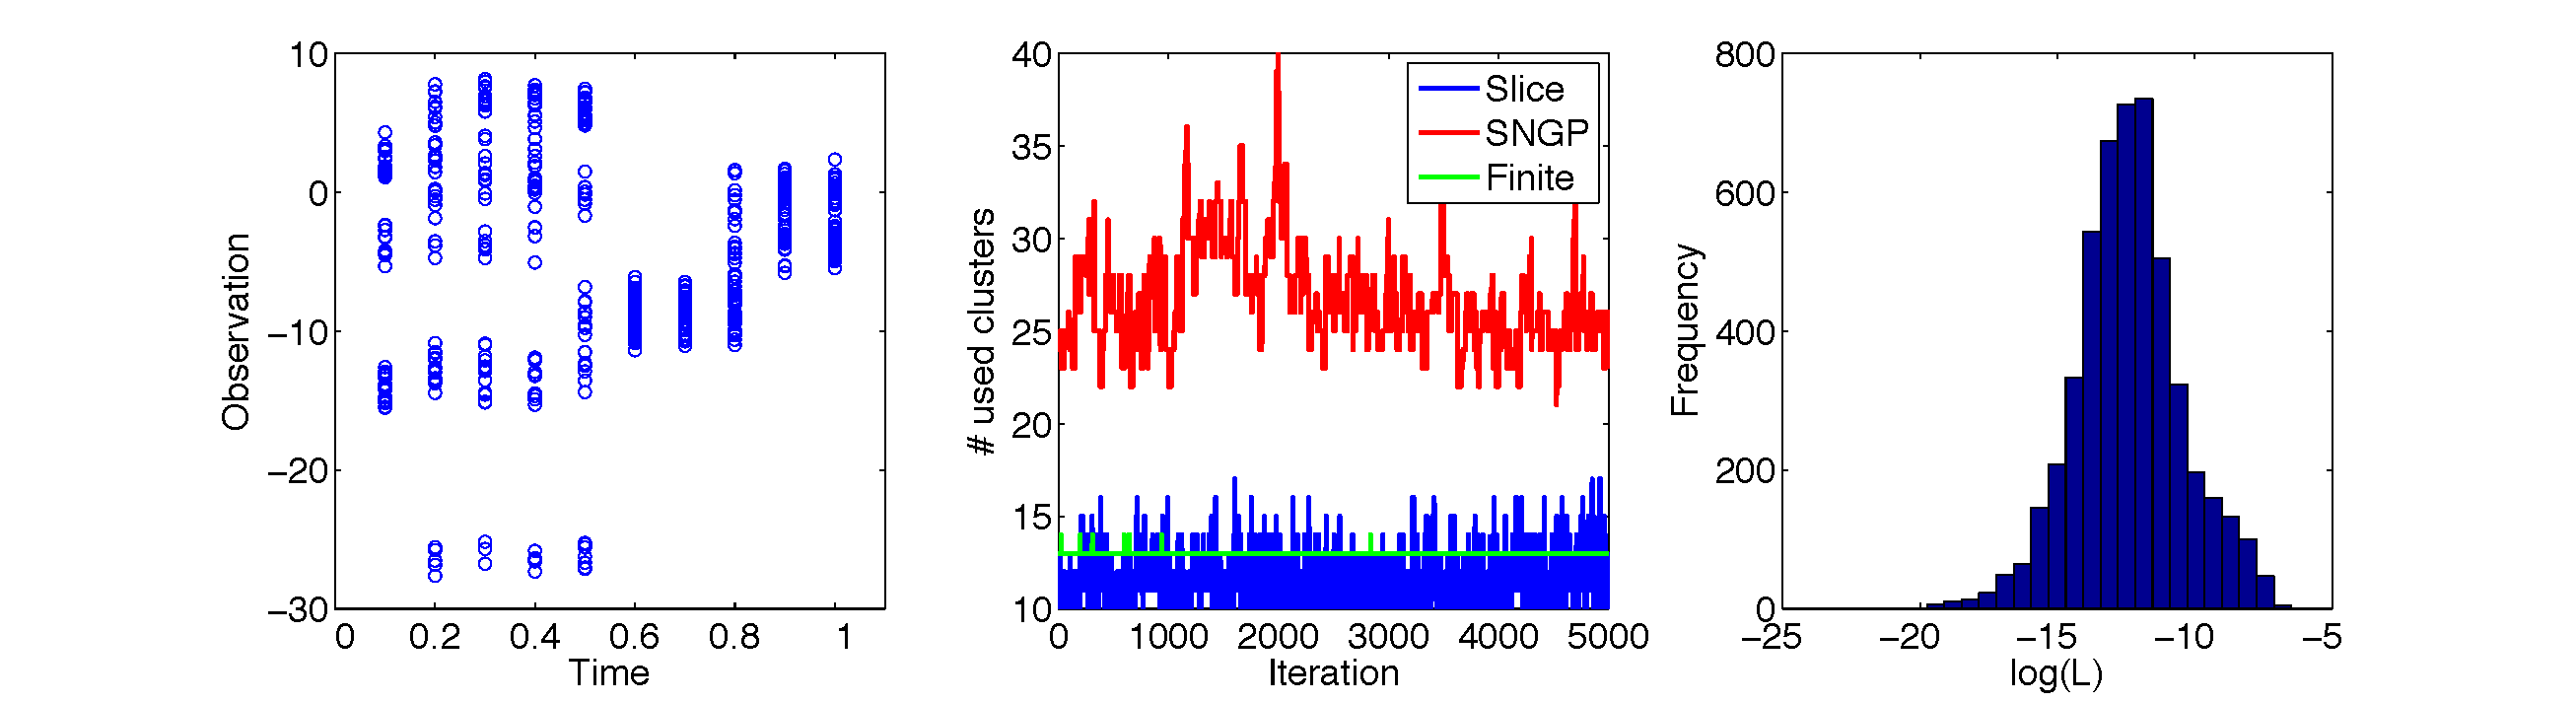
\includegraphics[scale=0.32]{figs/synth_stats.pdf}
  \end{center}
  \caption{Left: Synthetic data.  Middle: Trace plots of the number of clusters
  used by the three samplers.  Right: Histogram of truncation point $L$.
  }
  \label{fig:slicestats}
\end{figure}

We see that all three algorithms find a region of the posterior that gives
predictive estimates of a similar quality.  The autocorrelation estimates for 
the three samplers are also very similar. This might seem surprising, since the 
SNGP sampler uses sophisticated split-merge moves
to improve mixing, which have no analogue in the slice sampler. 
In addition, we note that although the per-iteration mixing performance is comparable, the average
time per $100$ iterations for the slice sampler was 
$\sim 10$ %$\sim 6$ 
seconds, for
the SNGP sampler was 
$\sim 30$ %$\sim 28$ 
seconds and for the finite sampler was 
$\sim 200$ %$\sim 194$ 
seconds. Even with only $100$ atoms the finite sampler
is much more expensive than the slice and SNGP\footnote{Sampling the cluster means
and assignments is the slowest step for the SNGP sampler taking about 3 seconds.
The times reported here only performed this step every 25 iterations
achieving reasonable results.  If this step were performed every iteration the
results may improve, but the computation time will explode.} samplers.

We also observe (Figure
\ref{fig:slicestats}) that both the slice and finite samplers
use essentially the true number of components underlying the data and that 
the SNGP sampler uses on average twice as many components.  The finite sampler finds a posterior mode with 13 clusters and rarely makes small moves from that
mode.  The slice sampler explores modes with 10-17 clusters, but never makes
large jumps away from this region.  The SNGP sampler explores the largest
number of used clusters ranging from 23-40, however, it has not explored
regions that use less clusters.

Figure \ref{fig:slicestats} also depicts the distribution
of the variable truncation level $L$ over all samples in the slice sampler. This suggests that a finite model that discards atoms with $\pi_k <
10^{-18}$ introduces negligible truncation error.  However, this value of $L$
corresponds to $\approx 10^{18}$ atoms in the finite model which is
computationally intractable.  To keep the computation times
reasonable we were only able to use $100$ atoms, a far cry
from the number implied by $L$.  

In Figure \ref{fig:preddens} (Left) we plot estimates of the predictive density
at each time stamp for the slice (a), finite (b) and SNGP (c) samplers.  All
three samplers capture the evolving structure of the distribution.  However,
the finite sampler seems unable to discard unneeded components.  This
is evidenced by the small mass of probability that spans times $[0,0.8]$ when
the data that the component explains only exists at times $[0.2,0.5]$.
The slice and SNGP samplers seem to both provide reasonable explanations for
the distribution, with the slice sampler tending to provide smoother estimates.

\subsection{Real data}
As well as providing an alternative inference method for existing models, our slice sampler can be used in a range of models that fall under the general class of KNRMs. To demonstrate this, we use the finite and slice versions of our sampler to learn two kernel DPs, one using a box kernel, $K(x,\mu) =
\idf{|x-\mu| < 0.2}$ (the setting in the SNGP), and the other using a square exponential kernel $K(x,\mu) = \exp(-200(x-\mu)^2)$, which has support
approximately on $[\mu-.2,\mu+.2]$.  The kernel was chosen to be somewhat
comparable to the box kernel, however, this kernel allows the influence of an
atom to diminish gradually as opposed to being constant. We compare to the SNGP sampler for the box kernel model, but note that this sampler is not applicable to the exponential kernel model.

We compare these approaches on two real-world datasets:
\begin{itemize}
  \item \textbf{Cosmic microwave background radiation (CMB)}\cite{Bennett:2003}: TT power spectrum measurements, $\eta$, from
the cosmic microwave background radiation (CMB) at various `multipole moments',
denoted $M$.  Both variables are
considered continuous and exhibit dependence.
We rescale $M$ to be in $[0,1]$ and standardize $\eta$ to have mean $0$ and
unit variance.
\item \textbf{Motorcycle crash data} \cite{Silverman:1985}.  This data set records the head acceleration, $A$, at various times
during a simulated motorcycle crash. We normalize time to $[0,1]$ and standardize $A$ to have
mean $0$ and unit variance.
\end{itemize}

Both datasets exhibit local heteroskedasticity, which cannot be captured using
the SNGP. For the CMB data, we consider only the first $600$ multipole moments, where the variance is approximately constant, allowing us to compare the SNGP sampler to the other algorithms. For all models we fixed the observation
variance to $0.02$, which we estimated from the standardized data.  To ease the 
computational burden of the samplers we picked $18$ time stamps in $[0.05,0.95]$,
equally spaced $0.05$ apart and assigned each observation to the time stamp
closest to its associated value of $M$.  This step is by no means necessary,
but the running time of the algorithms improves significantly. For the motorcycle data, there was no regime of constant variance, so we only compare the slice and finite
truncation samplers\footnote{The SNGP could still be used to model
this data, however, then we would be comparing the models as opposed to the
samplers.}.

For each dataset and each model/sampler, the held-out predictive log-likelihood, the mean number of used clusters and 
$\hat{\tau}$ are reported in  Table \ref{tab:mcmc}.  The
mixing characteristics of the chain are similar to those obtained for the
synthetic data.   We see in Table
\ref{tab:mcmc} that the box kernel and the square exponential kernel produce similar results on the CMB data. However, the kernel width was not optimized and different values may prove to yield superior results. For the motorcycle data we see a noticeable difference between using the box and square
exponential kernels where using the latter improves the held-out predictive
likelihood and results in both samplers using fewer components on average.

Figure \ref{fig:preddens} shows the predictive distributions obtained on the CMB data. Looking at the mean and $95\%$ CI of the predictive distribution (middle) we see that when using the box kernel the
SNGP actually fits the data the best.  This is most likely due to the fact that
the SNGP is using more atoms than the slice or finite samplers.  We show that the square exponential kernel (right) gives much smoother estimates and appears to fit the data
better, using the same number of atoms as were learned with the box kernel (see
Table \ref{tab:mcmc}).  We note that the slice sampler took 
$\sim 20$ %$\sim 14$
seconds per 100 iterations while the finite sampler used 
$\sim 150$ %$\sim 160$ 
seconds.  



%As with the CMB data we normalize time to $[0,1]$ and standardize $A$ to have
%mean $0$ and unit variance.  We use both the same box and square exponential
%kernels for this data as for the CMB dat.  We report the results in Table 
%\ref{tab:mcmc} where we see that for the box kernel the slice sampler has 
%found a region of the posterior with slightly better predictive likelihood.  In
%this case we see a noticeable difference between using the box and square
%exponential kernels where using the latter improves the held-out predictive
%likelihood and results in both samplers using fewer components on average.

\begin{figure}[t]
  \begin{center}
    \subfigure{
    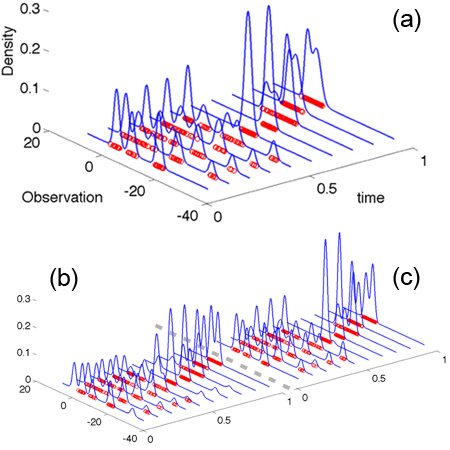
\includegraphics[bb=0 0 216 216,scale=0.5]{figs/synth_waterfall.pdf}
    }
    \subfigure{
    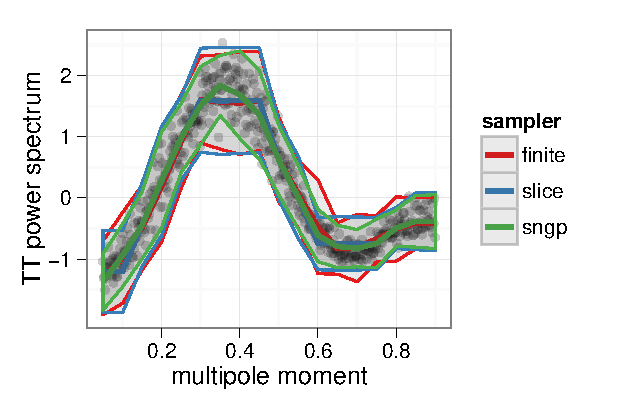
\includegraphics[bb=10 -15 300 184,scale=.48]{figs/cmb_box_predmean.pdf}
    }
    \subfigure{
    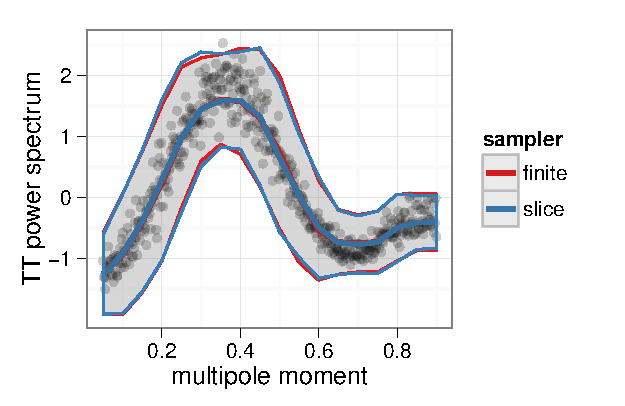
\includegraphics[bb=32 -15 300 184,scale=.48]{figs/cmb_se_predmean.pdf}
    }
  \end{center}
  \caption{\textbf{Left:} Predictive density at each time stamp for synthetic
  data using the slice (a), finite (b) and SNGP (c) samplers.  The scales of
  all three axis are identical.  \textbf{Middle:}
  Mean and $95\%$ CI of predictive distribution for all three
  samplers on CMB data using the box kernel.  \textbf{Right:} Mean and $95\%$
  CI of predictive distribution using the square exponential kernel.}
  \label{fig:preddens}
\end{figure}
